\section{Cavern $\gamma$ Generator}

\par
Although the LZ detector has been constructed underground to limit cosmic radiation, it does come with a drawback of being in a mine with a non-negligibly radioactive rock and the shotcreat and gravel within the David Cavern.
The rate of this has been measured and can be attributed to the shotcreat and gravel. 

One of the most significant sources of background come not from any internal component but rather from $^{238}U$, $^{232}Th$ and $^{40}K$ decays from the cavern in which the LZ detector exists \cite{LZ_Gamma_Ray_Background_ref}.




\par
For the creation of the generator additional cavern properties are added to the simulation.
Namely; a steel pyramid and gravel beneath the water tank, and the cavern gamma. 
These adaptions are shown in Figure \ref{fig:Cavern_Geometry}.

\begin{figure}[!htbp]
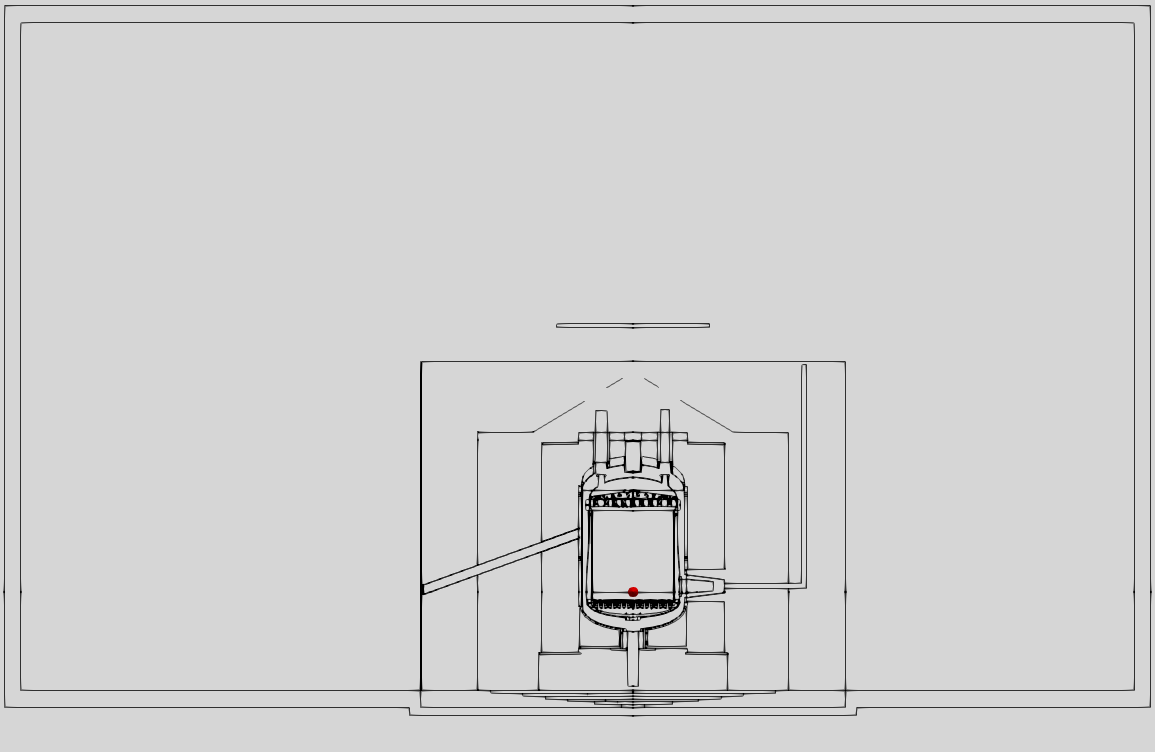
\includegraphics[width=\textwidth]{Figures/Simulations/cavern_geometry_2.png}
\centering
\caption{Cavern Geometry}
\label{fig:Cavern_Geometry}
\end{figure}

\par
Given the measured rate in the .


\par
In short, this means that every $\gamma$ in the generator represents 130000 $\gamma$'s from the rock, and so is a significant computational saving.
